

\begin{table}\caption{This table compares the analytical values for L=2 with the numerical ones after $10^6$ Monte Carlo cycles. The values are in units per spin.}\label{tab:compare_values}
\begin{tabular}{ccc}
& Numerical: & Analytical:\\ \hline
$\left<E\right>$ &   -1.9958 & -1.9960\\
$\left<E^2\right>$ &   15.9664 & 15.9679\\
$\left<M\right>$ &    0.0451 & 0\\
$\left<M^2\right>$ &    3.9930 & 3.9933\\
$\left<|M|\right>$ &    0.9986 & 0.9987\\
$\chi$ &   3.9849 & 3.9933\\
  $C_V$& 0.0335 & 0.0321\\
\end{tabular}
\end{table}

\begin{figure}[H]
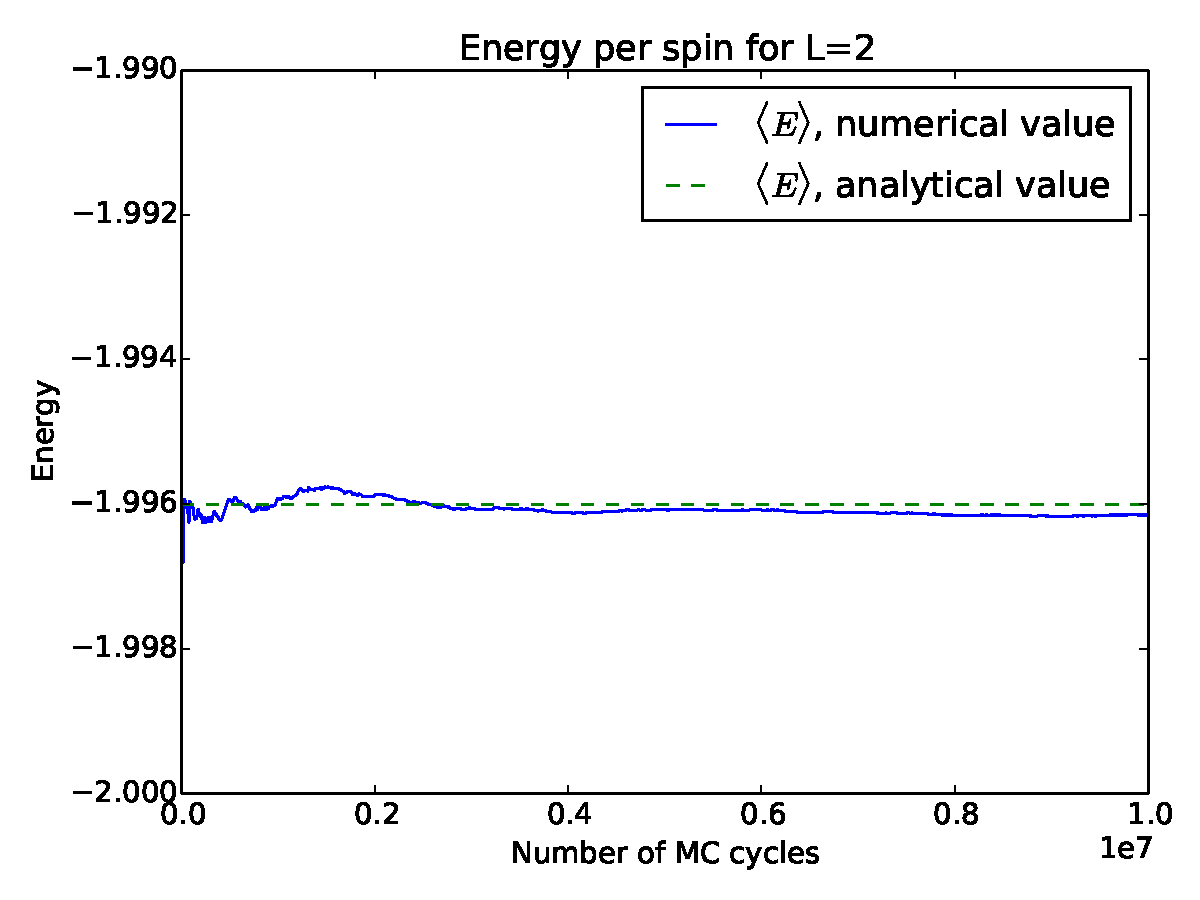
\includegraphics[width=\linewidth]{../results/4b/L_2_energy}\caption{This is a plot of the expectation value of the energy per spin verus number of Monte Carlo cycles. The plot shows that at least $ 9 \cdot 10^{5} $ MC cycles are necessary for a good argeement.}\label{fig:L_2_energy}
\end{figure}

\begin{figure}[H]
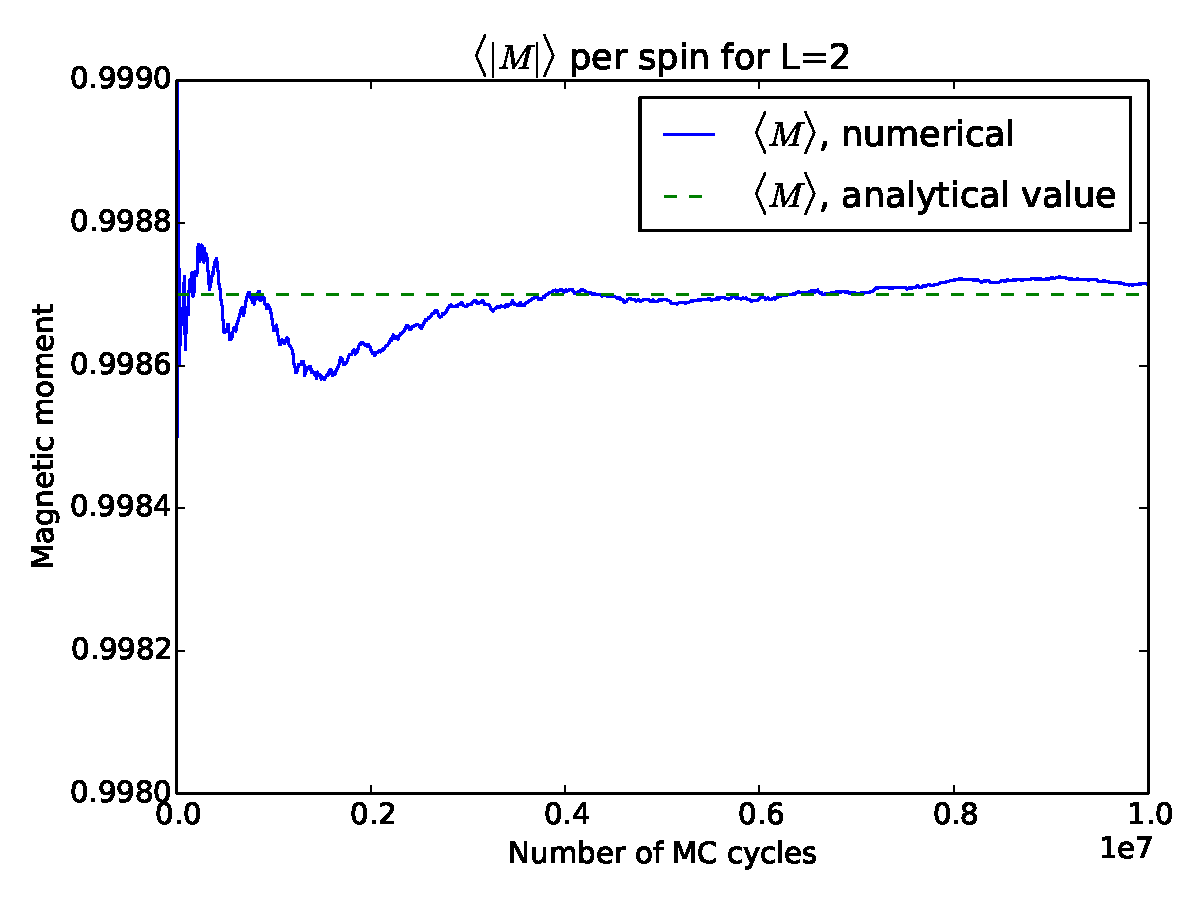
\includegraphics[width=\linewidth]{../results/4b/L_2_magnetic_abs}\caption{This is a plot of the expectation value of the mean absolute value of the magnetic moment per spin verus number of Monte Carlo cycles. The plot shows that at least $ 8 \cdot 10^{5} $ MC cycles are necessary for a good argeement, but all the way to $10^6$ the value is a bit low.}\label{fig:L_2_magnetic_abs}
\end{figure}

\begin{figure}[H]
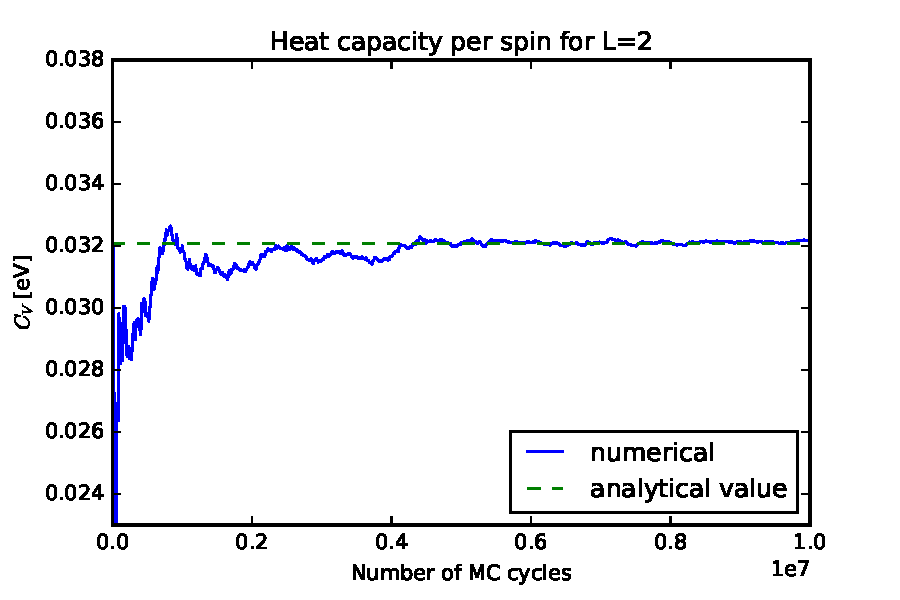
\includegraphics[width=\linewidth]{../results/4b/L_2_heat_capasity}\caption{This is a plot of the heat capacity per spin verus number of Monte Carlo cycles. The plot shows that at least $ 6 \cdot 10^{5} $ MC cycles are necessary for a good argeement.}\label{fig:L_2_heat_capacity}
\end{figure}

\begin{figure}[H]
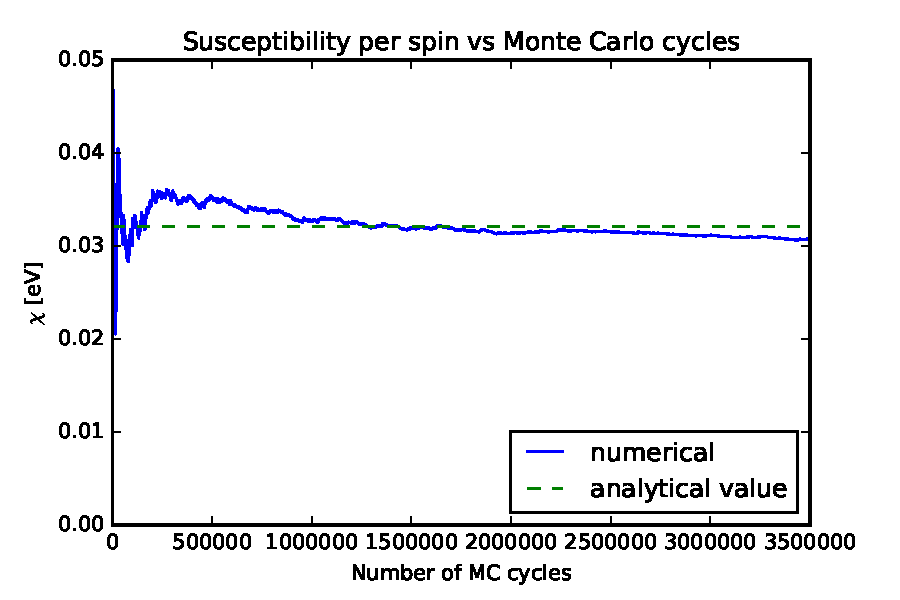
\includegraphics[width=\linewidth]{../results/4b/L_2_susceptibility}\caption{This is a plot of the susceptibility per spin verus number of Monte Carlo cycles. The plot shows that at least $ 6 \cdot 10^{5} $ MC cycles are necessary for a good argeement.}\label{fig:L_2_susceptibility}
\end{figure}